\documentclass[../thesis.tex]{subfiles}

\begin{document}

\section{Thu thập và xử lý dữ liệu}

Chúng tôi sử dụng lại một phần tập dữ liệu mà chúng tôi đã thu thập từ nghiên cứu trước \cite{faster-rcnn-nngbao-dldien}. Bên cạnh đó, chúng tôi cũng thu thập bổ sung dữ liệu biển báo sử dụng camera hành trình để cải tiến hiệu quả của giải thuật học. Chúng tôi đã tiến hành lược bỏ một số loại biển báo không quan trọng như trạm xăng, trạm xe buýt, chợ,\ldots\ và gom nhóm các loại biển báo có ý nghĩa tương tự nhau, cụ thể là:

\begin{itemize}[topsep=0pt]
    \item Nhiều chỗ ngoặt nguy hiểm liên tiếp (202): gồm các biển báo 202a, 202b.
    \item Đường hẹp (203): gồm các biển báo 203a, 203b, 203c.
    \item Đường giao nhau cùng cấp (205): gồm các biển báo 205a, 205b, 205c, 205d, 205e.
    \item Giao nhau với đường không ưu tiên (207): gồm các biển báo 207a, 207b, 207c, 207d.
    \item Đường người đi bộ sang ngang (423): gồm các biển báo 423a, 423b.
\end{itemize} 

Từ các đoạn video được quay từ camera hành trình, chúng tôi tách lấy các đoạn chứa biển báo và lấy ra những khung ảnh tốt dùng cho việc huấn luyện mô hình. Tập dữ liệu được chia thành 2 tập con, tập huấn luyện (training set) và tập đánh giá (test set) với tỉ lệ là 80:20.

Các ảnh sau quá trình tiền xử lý đều được gán nhãn bằng phần mềm labelImg \cite{labelImg}. Thông tin chi tiết về nhãn của các loại biển báo được cho trong Bảng \ref{Table:datset}\footnote{Có một số loại biển báo xuất hiện cùng nhau trong một bức ảnh nên những thống kê trên đây chỉ mang tính chất tương đối, không hoàn toàn chính xác về số lượng các loại biển báo trong tập dữ liệu.}.

\begin{longtable}{| c | l | l | c | c |}
    \hline
    \thead{STT} & \thead{Nhãn} & \thead{Mô tả} & \thead{Train} & \thead{Test}\\
    \hline
    1 & 102 & Cấm đi ngược chiều & 83 & 22\\
    \hline
    2 & 130 & Cấm dừng xe và đỗ xe & 268 & 60\\
    \hline 
    3 & 131 & Cấm đỗ xe & 180 & 54\\
    \hline
    4 & 201a & Chỗ ngoặt nguy hiểm vòng bên trái & 94 & 27\\
    \hline
    5 & 201b & Chỗ ngoặt nguy hiểm vòng bên phải & 97 & 29\\
    \hline
    6 & 202 & Nhiều chỗ ngoặt nguy hiểm liên tiếp & 158 & 33\\
    \hline
    7 & 203 & Đường hẹp & 53 & 16\\
    \hline
    8 & 205 & Đường giao nhau cùng cấp & 307 & 78\\
    \hline 
    9 & 207 & Giao nhau với đường không ưu tiên & 570 & 146\\
    \hline
    10 & 208 & Giao nhau với đường ưu tiên & 145 & 29\\
    \hline
    11 & 209 & Giao nhau có tín hiệu đèn & 107 & 23\\
    \hline
    12 & 221 & Đường có sóng mấp mô nhân tạo & 97 & 16\\
    \hline
    13 & 224 & Người đi bộ cắt ngang & 407 & 97\\
    \hline
    14 & 225 & Trẻ em & 336 & 95\\
    \hline
    15 & 233 & Nguy hiểm khác & 88 & 18\\
    \hline
    16 & 245 & Đi chậm & 62 & 12\\
    \hline
    17 & 302 & Đi bên phải & 125 & 27\\
    \hline
    18 & 303 & Nơi giao nhau chạy theo vòng xuyến & 108 & 22\\
    \hline
    19 & 423 & Đường người đi bộ sang ngang & 307 & 90\\
    \hline
    20 & crowded & Khu đông dân cư & 50 & 9\\
    \hline
    21 & end\_crowded & Hết khu đông dân cư & 29 & 8\\ 
    \hline
    22 & traffic\_light & Đèn giao thông & 143 & 43\\
    \hline
    \multicolumn{3}{|c|}{\textbf{Tổng}} & \textbf{3814} & \textbf{954}\\
    \hline
    \caption{Thông tin về tập dữ liệu}
    \label{Table:datset}
\end{longtable}

\section{Thiết kế mô hình}

Chúng tôi sử dụng lại kiến trúc mô hình YOLOv3 phiên bản rút gọn, kiến trúc này bao gồm 13 lớp tích chập, xen kẻ là các lớp max-pooling. Mô hình YOLOv3 rút gọn kết hợp 2 lưới có kích thước là $13 \times 13$ và $26 \times 26$\footnote{Mô hình đầy đủ có thêm một lưới $52 \times 52$} để cải tiến kết quả nhận dạng so với các phiên bản trước của YOLO. Giữa 2 lớp YOLO ứng với 2 lưới $13 \times 13$ và $26 \times 26$ là các lớp \textit{route}\footnote{Điều hướng vector đầu vào cho lớp tiếp theo là một lớp ở trước đó.} và \textit{upsample}\footnote{Tăng kích cỡ vector đặc trưng để nhận dạng ở lớp YOLO tiếp theo.}.

Để mô hình có thể đáp ứng được số lớp trong tập dữ liệu mà chúng tôi đã thu thập, chúng tôi chỉnh sửa số lượng filter ở 2 lớp tích chập phía trước mỗi lớp YOLO, số filter này chính là chiều sâu của vector đặc trưng, do đó số lượng filter phải đáp ứng là:

$\text{Số filter} = \left(\text{số lớp} + 5\right) \times \text{số anchor} = \left(\text{22} + 5\right) \times \text{3} = 81$.

Trong đó, 5 chính là các giá trị $b_x$, $b_y$, $b_w$, $b_h$ và $p$.

Ngoài ra, kích thước các anchor box được chọn bằng duyệt qua toàn bộ tập dữ liệu và sử dụng giải thuật \textit{k-means} để phân cụm kích thước của tất cả các khung chứa đối tượng. Kết quả sau khi phân cụm đã chọn được các anchor có kích thước như sau: (20, 39), (51, 28), (37, 72), (89, 48), (116, 61), (180, 95).

\begin{figure}[H]
    \centering
    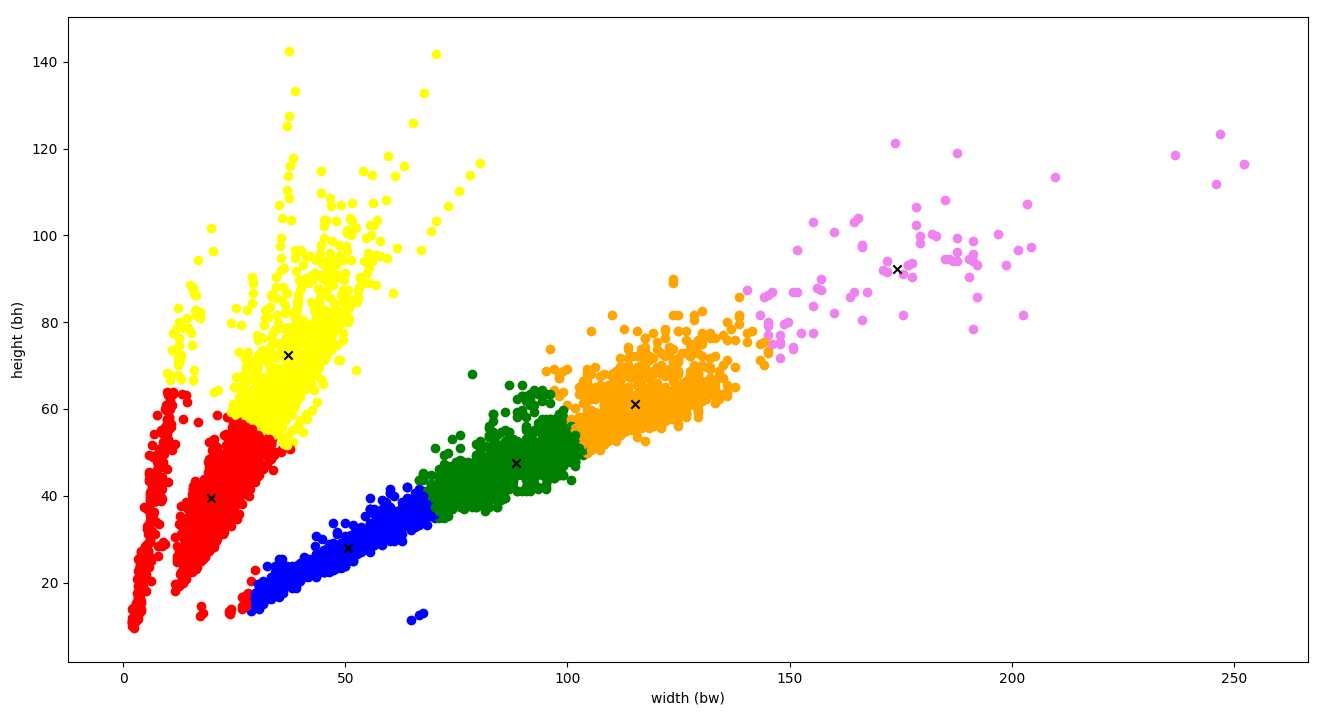
\includegraphics[width=\linewidth]{images/6_anchors.png}
    \caption{Kết quả phân cụm để chọn anchor cho tập dữ liệu bằng giải thuật \textit{k-means}}
    \label{6_anchors}
\end{figure}

\section{Huấn luyện mô hình}

Mô hình được huấn luyện trên một máy chủ ảo 48 cores, RAM 192GB (không có GPU) trong vòng 2 tuần với kích thước mỗi \textit{batch} là 128 ảnh. Mô hình hội tụ sau hơn 30 epochs (4000 steps).

\end{document}